% Mustafa Alparslan
%X: book Ceyhun
%ZZZ: page 180.
%\documentclass[fleqn]{book}
\documentclass[11pt]{amsbook}

\usepackage[turkish]{babel}
\usepackage{../Ceyhun}	
\usepackage{../amsTurkish}

\begin{document}
% ++++++++++++++++++++++++++++++++++++++
\hPage{180}
% ++++++++++++++++++++++++++++++++++++++

 \begin{figure}[h]
 \centering
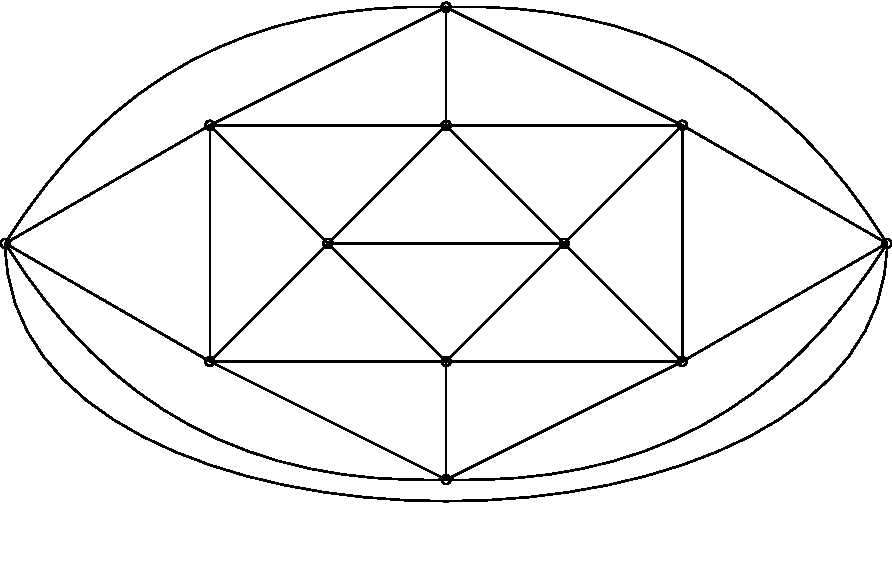
\includegraphics[width=0.90\textwidth]{images/cyhn180fig01.pdf} 
\label{fig:cyhn-180-fig01}
\caption{12 düğümlü dönüşül düzlemsel bir çizge.}
\end{figure}

çizgelerin bir çokyüzlü olark düşünülebileceği sonucuna varabiliriz. Öyleyse bu gözlem üzerinde biraz daha duralım. $Ç(d,a)$ da kertesi i olan düğümlerin sayısını $d_i$ ve $i$ sayıda ayrıtla çevrili yüzeylerin sayısını ise $y_i$ ile gösterelim. Bir yüz en az üç ayrıtla tanımlanabileceğinden, 
\begin{align*}
 2a =& \sum_{i \geq 3} \: i \: d_{i} \\
    =& \sum_{i \geq 3} \: i \: y_{i}
\end{align*}
yazabiliriz.
\begin{theorem}
Çokyüzlünün en az bir yüzü, 
\end{theorem} 
\end{document}